\documentclass[a4paper,12pt]{report}

\usepackage{../courslatex}
\usepackage{exos}
\usepackage{enumitem}

\setlist[enumerate]{align=left,leftmargin=1cm,itemsep=5pt,parsep=0pt,topsep=0pt,rightmargin=0.5cm}

\setlist[itemize]{align=left,labelsep=1em,leftmargin=*,itemsep=0pt,parsep=0pt,topsep=0pt,rightmargin=0cm}

\renewcommand{\titreChapitre}{Ch4~: Équations du premier degré à une inconnue} 
\renewcommand{\numeroSerie}{9}

\begin{document}
\vspace*{-2\baselineskip}
\textLigne{Activités}
\begin{acti}
Compléter les équations $b), c)$ et $d)$ pour obtenir des équations équivalentes à l'équation $A$.
	\begin{tasks}(4)
\task $x=\dfrac{2}{5} y-2$
\task $5 x=\ldots$
\task $x+2=\ldots$
\task $\dfrac{5}{2} x=\ldots$
	\end{tasks}
\end{acti}
\begin{acti}
Résoudre les équations entièrement de tête.
	\begin{tasks}(4)
\task $4 x=9 x$
\task $6 x+3=5 x$
\task $4 x-5=3 x+2$
\task $8 x=9 x+3$
\task $4 x-7=10 x-7$
\task $5 x+1=5 x-1$
\task $5+2 x=4 x-5$
\task $7 x-8=-x$
\task $3 x-1=3 x-1$
\task $13 x-1=5 x-2$
\task $6 x+4=2 x+10$
\task $2-5 x=11-3 x$
	\end{tasks}
\end{acti}
\begin{acti}
Traduire chaque phrase par une équation, puis résoudre.
	\begin{tasks}
		\task \enquote{Le triple du nombre $x$ vaut 2 de plus que $x$.}
		\task \enquote{La somme de $x$ et de 3 vaut 2 de moins que le double de $x$.}
	\task \enquote{Le double d'un nombre dépasse ses deux tiers de 10.}
\task \enquote{Si l'on soustrait le dixième de $x$ au quart de $x$ on obtient 2 de moins que $x$.}
\task \enquote{Si l'on retranche 5 du triple de $x$, on obtient la moitié de la somme de 3 et de $x$.}
	\end{tasks}
\end{acti}
\begin{acti}
Sur le dessin ci-dessous, la figure ombrée est un carré, et le grand quadrilatère, un rectangle.

(Toutes les longueurs sont en cm.)

\hfill
\begin{minipage}[t]{0.5\textwidth}{
\vspace{0pt}
\begin{tikzpicture}
    \tkzDefPoint[label=below:{}](-1,-1){A}
    \tkzDefPoint[label=right:{}](-1,1){B}
    \tkzDefPoint[label=above:{}](2,0.5){C}
    \tkzDefPoint[label=above:{}](3,0.5){D}
    \tkzDefPoint[label=above:{}](2,-1){G}
    \tkzDefPoint[label=above:{}](3,1){E}
    \tkzDefPoint[label=above:{}](3,-1){F}

    \tkzDrawPolygon(A,B,E,F)
    \tkzDrawPolygon(F,G,C,D)
    \tkzFillPolygon[pattern=north west lines](F,G,C,D)
    \tkzDrawSegment[dashed,dim={$2$,15pt,right=2mm,midway,font=\footnotesize}](E,D)
    \tkzDrawSegment[dashed,dim={$x$,-15pt,right=2mm,midway,font=\footnotesize}](F,D)
    \tkzDrawSegment[dashed,dim={$6$,-15pt,below=2mm,midway,font=\footnotesize}](A,G)


\end{tikzpicture}
}
\end{minipage}
\begin{minipage}[t]{0.4\textwidth}{
\vspace{0pt}
Déterminer $x$ pour que l'aire de la partie blanche soit égale à $38 \mathrm{~cm}^2$.
}
\end{minipage}

\end{acti}

\begin{acti}
Trouver dans chaque cas quel nombre mettre au départ pour retrouver le même nombre après un tour de circuit.
\begin{tasks}(2)
	\task 

	\begin{tikzpicture}
        [
        squarednode/.style={%
            rectangle,
            draw=black!60,
            fill=white,
            very thick,
            minimum size=5mm,
            text centered,
            text width=0.2cm,
            text height=0.2cm,
            node distance=1cm
        }
        ]
        %Nodes
        \node[squarednode]      (e4)                             {};
        \node[squarednode]      (e1)       [above=of e4]       {};
        \node[squarednode]      (e3)  [right= of e4] {};
        \node[squarednode]      (e2)     [above=of e3]   {};
	 \node[node distance = 0.1cm] (e5)[above=of e1] {départ};      
	 \node[node distance = 0.1cm] (e5)[left=of e1] {arrivée};      
        %Lines
        \draw[->] (e1.east) -- node [above,midway] {$+2$} (e2.west);
        \draw[<-] (e1.south) -- node [left,midway] {$\cdot 7$}(e4.north);
        \draw[<-] (e3.north) -- node [right,midway] {$\cdot 3$}(e2.south);
        \draw[<-] (e4.east) -- node [above,midway] {$-5$} (e3.west);
        \end{tikzpicture}
	\task 

	\begin{tikzpicture}
        [
        squarednode/.style={%
            rectangle,
            draw=black!60,
            fill=white,
            very thick,
            minimum size=5mm,
            text centered,
            text width=0.2cm,
            text height=0.2cm,
            node distance=1cm
        }
        ]
        %Nodes
        \node[squarednode]      (e4)                             {};
        \node[squarednode]      (e1)       [above=of e4]       {};
        \node[squarednode]      (e3)  [right= of e4] {};
        \node[squarednode]      (e2)     [above=of e3]   {};
	 \node[node distance = 0.1cm] (e5)[above=of e1] {départ};      
	 \node[node distance = 0.1cm] (e5)[left=of e1] {arrivée};      
        %Lines
        \draw[->] (e1.east) -- node [above,midway] {$\cdot 2$} (e2.west);
        \draw[<-] (e1.south) -- node [left,midway] {$+3$}(e4.north);
        \draw[<-] (e3.north) -- node [right,midway] {$- 1$}(e2.south);
        \draw[<-] (e4.east) -- node [above,midway] {$\cdot 5$} (e3.west);
        \end{tikzpicture}

 
\end{tasks}
        	\begin{tasks}
A. $\square$ B.
B.
C. $1=\frac{x}{4}-\frac{3 x}{8}$
	\end{tasks}
\end{acti}
\begin{acti}
Résoudre les équations dans $\mathbb{R}$.
	\begin{tasks}(4)
\task $\dfrac{x}{2}+\dfrac{x}{3}=\dfrac{5}{6}$
\task $\dfrac{x}{3}+\dfrac{4}{5}=\dfrac{5}{6}$
\task $\dfrac{x-15}{5}-\dfrac{4-3 x}{4}=15$
\task $x+\dfrac{x}{6}-\dfrac{x}{3}=3$
\task $\dfrac{2 x}{3}-\dfrac{4 x}{9}=\dfrac{3}{5} \cdot \dfrac{x}{2}$
\task $\dfrac{x+1}{4}-\dfrac{x-1}{3}=0$
\task $\dfrac{x+3}{5}+\dfrac{x+3}{4}=\dfrac{9}{5}$
\task $\dfrac{x}{4}-\dfrac{x}{8}=\dfrac{3}{24} x-1$
	\end{tasks}
\end{acti}

\textLigne{Exercices}
\textLigne{Automatismes}

\end{document}

